% !TEX TS-program = pdflatex
% !TEX encoding = UTF-8 Unicode

% This is a simple template for a LaTeX document using the "article" class.
% See "book", "report", "letter" for other types of document.

\documentclass[11pt]{article} % use larger type; default would be 10pt

\usepackage[utf8]{inputenc} % set input encoding (not needed with XeLaTeX)

%%% Examples of Article customizations
% These packages are optional, depending whether you want the features they provide.
% See the LaTeX Companion or other references for full information.

%%% PAGE DIMENSIONS
\usepackage{geometry} % to change the page dimensions
\geometry{a4paper} % or letterpaper (US) or a5paper or....
% \geometry{landscape} % set up the page for landscape
%   read geometry.pdf for detailed page layout information

\usepackage{graphicx} % support the \includegraphics command and options

% \usepackage[parfill]{parskip} % Activate to begin paragraphs with an empty line rather than an indent

%%% PACKAGES
\usepackage{booktabs} % for much better looking tables
\usepackage{array} % for better arrays (eg matrices) in maths
%\usepackage{paralist} % very flexible & customisable lists (eg. enumerate/itemize, etc.)
%TODO uncomment paralist
\usepackage{verbatim} % adds environment for commenting out blocks of text & for better verbatim
\usepackage{subfig} % make it possible to include more than one captioned figure/table in a single float
% These packages are all incorporated in the memoir class to one degree or another...

\usepackage{float}
\usepackage{tabularx}
\usepackage{color}
\usepackage{xcolor}
\usepackage{listings}
\usepackage{caption}
\DeclareCaptionFont{white}{\color{white}}
\DeclareCaptionFormat{listing}{\colorbox{gray}{\parbox{\textwidth}{#1#2#3}}}
\captionsetup[lstlisting]{format=listing,labelfont=white,textfont=white}



\def\worksheet#1#2{%
  \begin{center}
  {\large\bf #1} \\
  {\normalsize\bf #2} \\[12pt]
  \begin{footnotesize}
  \input work-sheets-in-latex/#1.tex
  \end{footnotesize}
  \end{center}  
  \vfill}

\renewcommand\appendix{\par
  \setcounter{section}{0}
  \setcounter{subsection}{0}
  \setcounter{figure}{0}
  \setcounter{table}{0}
  \renewcommand\thesection{Appendix \Alph{section}}
  \renewcommand\thefigure{\Alph{section}\arabic{figure}}
  \renewcommand\thetable{\Alph{section}\arabic{table}}
}

%%% HEADERS & FOOTERS
\usepackage{fancyhdr} % This should be set AFTER setting up the page geometry
\pagestyle{fancy} % options: empty , plain , fancy
\renewcommand{\headrulewidth}{0pt} % customise the layout...
\lhead{}\chead{}\rhead{}
\lfoot{}\cfoot{\thepage}\rfoot{}

%%% SECTION TITLE APPEARANCE
%\usepackage{sectsty}
%TODO uncomment sectsty
%\allsectionsfont{\sffamily\mdseries\upshape} % (See the fntguide.pdf for font help)
% (This matches ConTeXt defaults)

%%% ToC (table of contents) APPEARANCE
%\usepackage[nottoc,notlof,notlot]{tocbibind} % Put the bibliography in the ToC
%TODO uncomment tocbibind
%\usepackage[titles,subfigure]{tocloft} % Alter the style of the Table of Contents
%\renewcommand{\cftsecfont}{\rmfamily\mdseries\upshape}
%\renewcommand{\cftsecpagefont}{\rmfamily\mdseries\upshape} % No bold!

%%% END Article customizations

%%% The "real" document content comes below...

\title{easyAround}
\author{Marco De Nadai, Claudia Minardi}
%\date{} % Activate to display a given date or no date (if empty),
         % otherwise the current date is printed 

\begin{document}
\maketitle

\section{Introduction}
This document illustrates the process of the development of an information system according to the CommonKADS approach. \\
The idea at the base of the project is to build a system capable of assisting a Travel Agent in satisfying the customers. The software must be able to exploit the knowledge of the Travel Agent in order to build a customized itinerary that reflect the desire of the client. \\
To do so, it is necessary to have precise knowledge rules embedded inside the system itself: this can be done by building a series of models that will constitute the core structure of the software. \\
The final piece of software, namely \textit{easyAround} will be able to:
\begin{itemize}
\item Classify customers according to their age and physical capabilities;
\item Gather information on each customer's preferences and personal taste;
\item Gather specific information on each customer's desire for a specific trip;
\item Propose to each customer an ideal trip, based on the gathered information;
\item Let the customers revise and personalize their own itinerary;
\end{itemize}
The target domain of the software resides inside one single city: the final itineary will be composed of locations to be visited inside that particular city, according to a standard timetable possessed by the Travel Agency. \\
The target user of the software is the Travel Agent appointed with the task of creating cusomized itineraries for clients who travel alone or accompanied by children.
\newpage
\section{Context Knowledge}
\worksheet{OM-1}{Identifying knowledge-oriented problems and
opportunities in the organization}
\worksheet{OM-2}{Description of organizational aspects that
have an impact on and/or are affected by chosen knowledge solutions}
\begin{figure}[H]
\centering
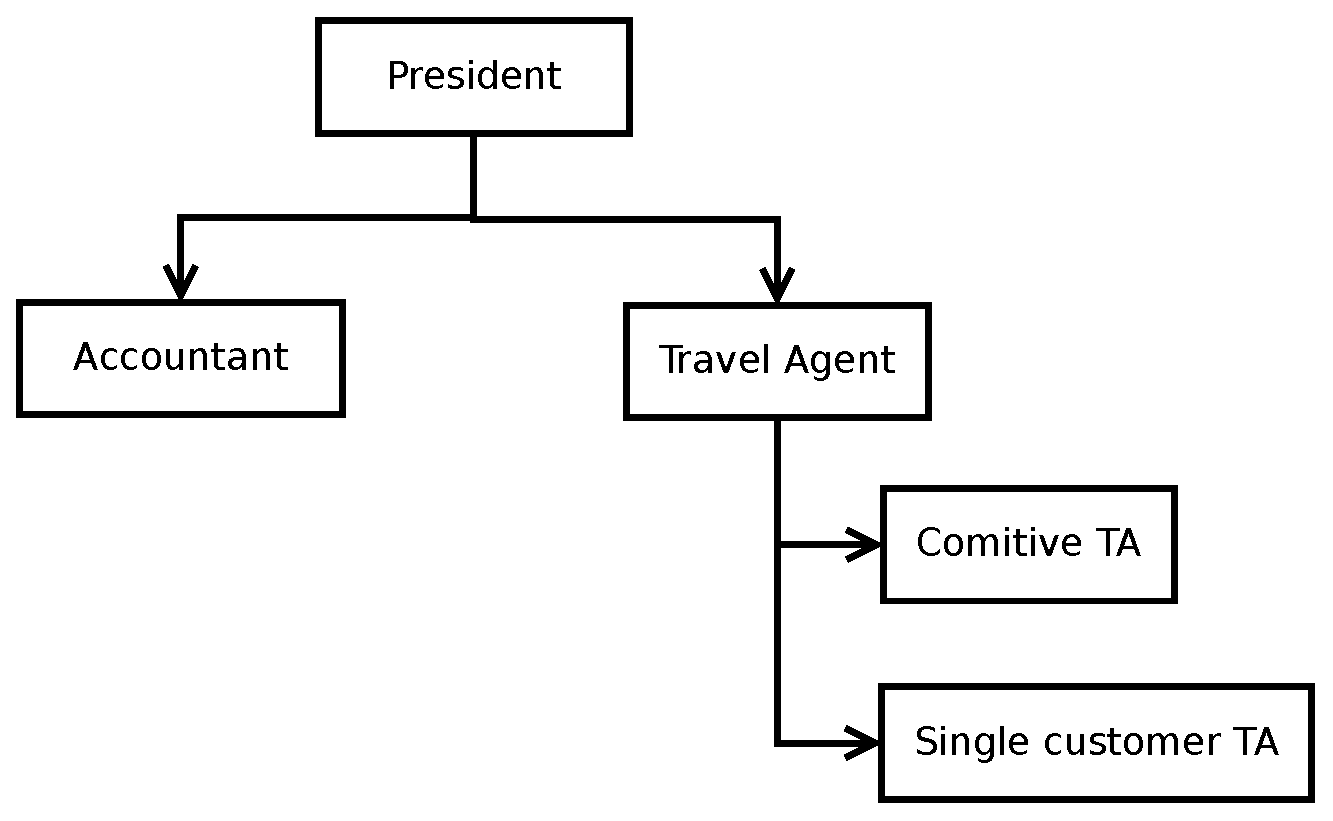
\includegraphics[width=10cm]{images/azienda.eps}
\caption{Organization structure}
\label{fig:orgStructure}
\end{figure}
\begin{figure}[H]
\centering
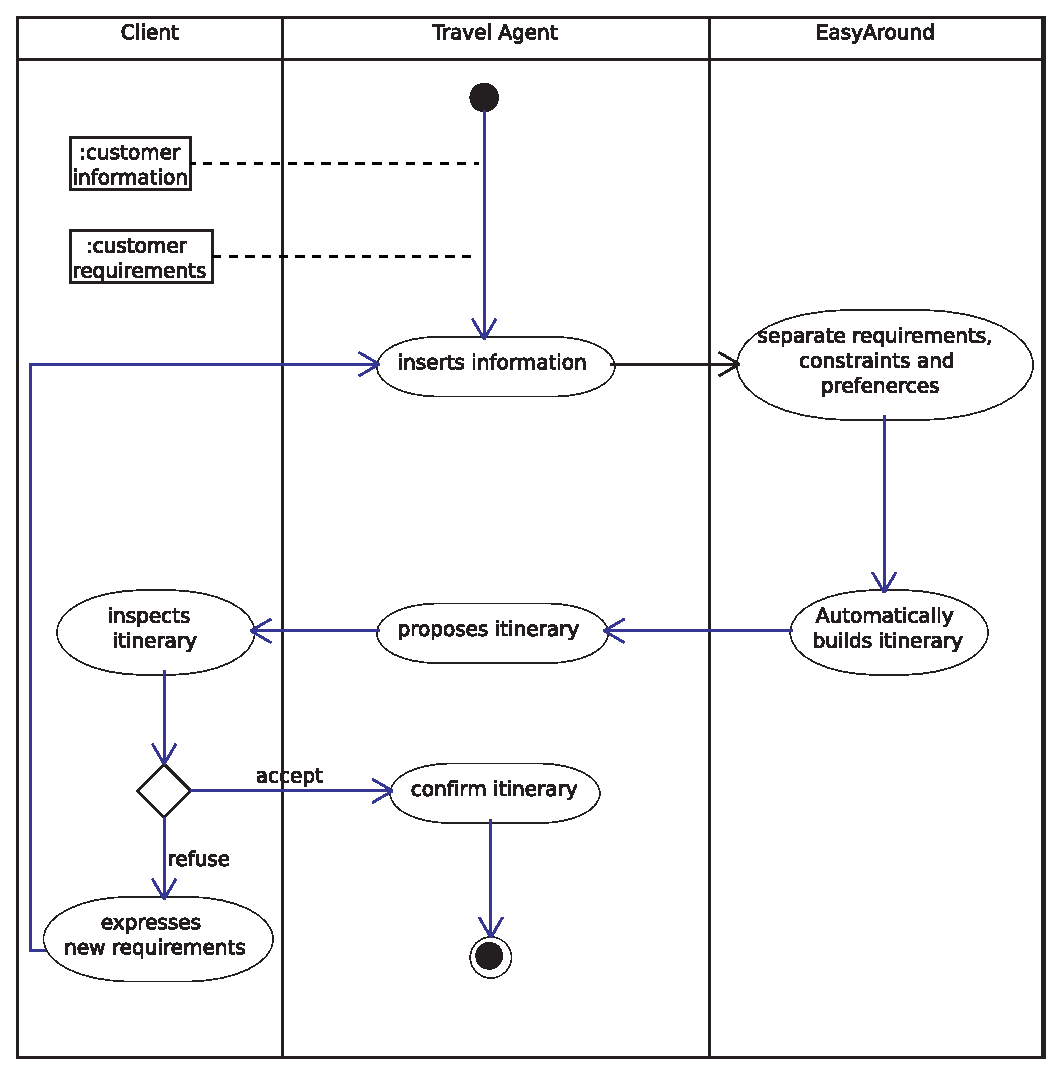
\includegraphics[width=\textwidth]{images/activity.eps}
\caption{Organization process}
\label{fig:orgProcess}
\end{figure}
\worksheet{OM-5}{Checklist for the feasibility decision
document}
\worksheet{TM-1}{Refined description of the tasks within the
target process}
\worksheet{TM-2}{Specification of the knowledge employed for a
task, and possible bottlenecks and areas for improvement}
\worksheet{AM-1}{Agent specification according to the
CommonKADS agent model}

\clearpage
\section{Task Knowledge}

\begin{figure}[h]
\centering
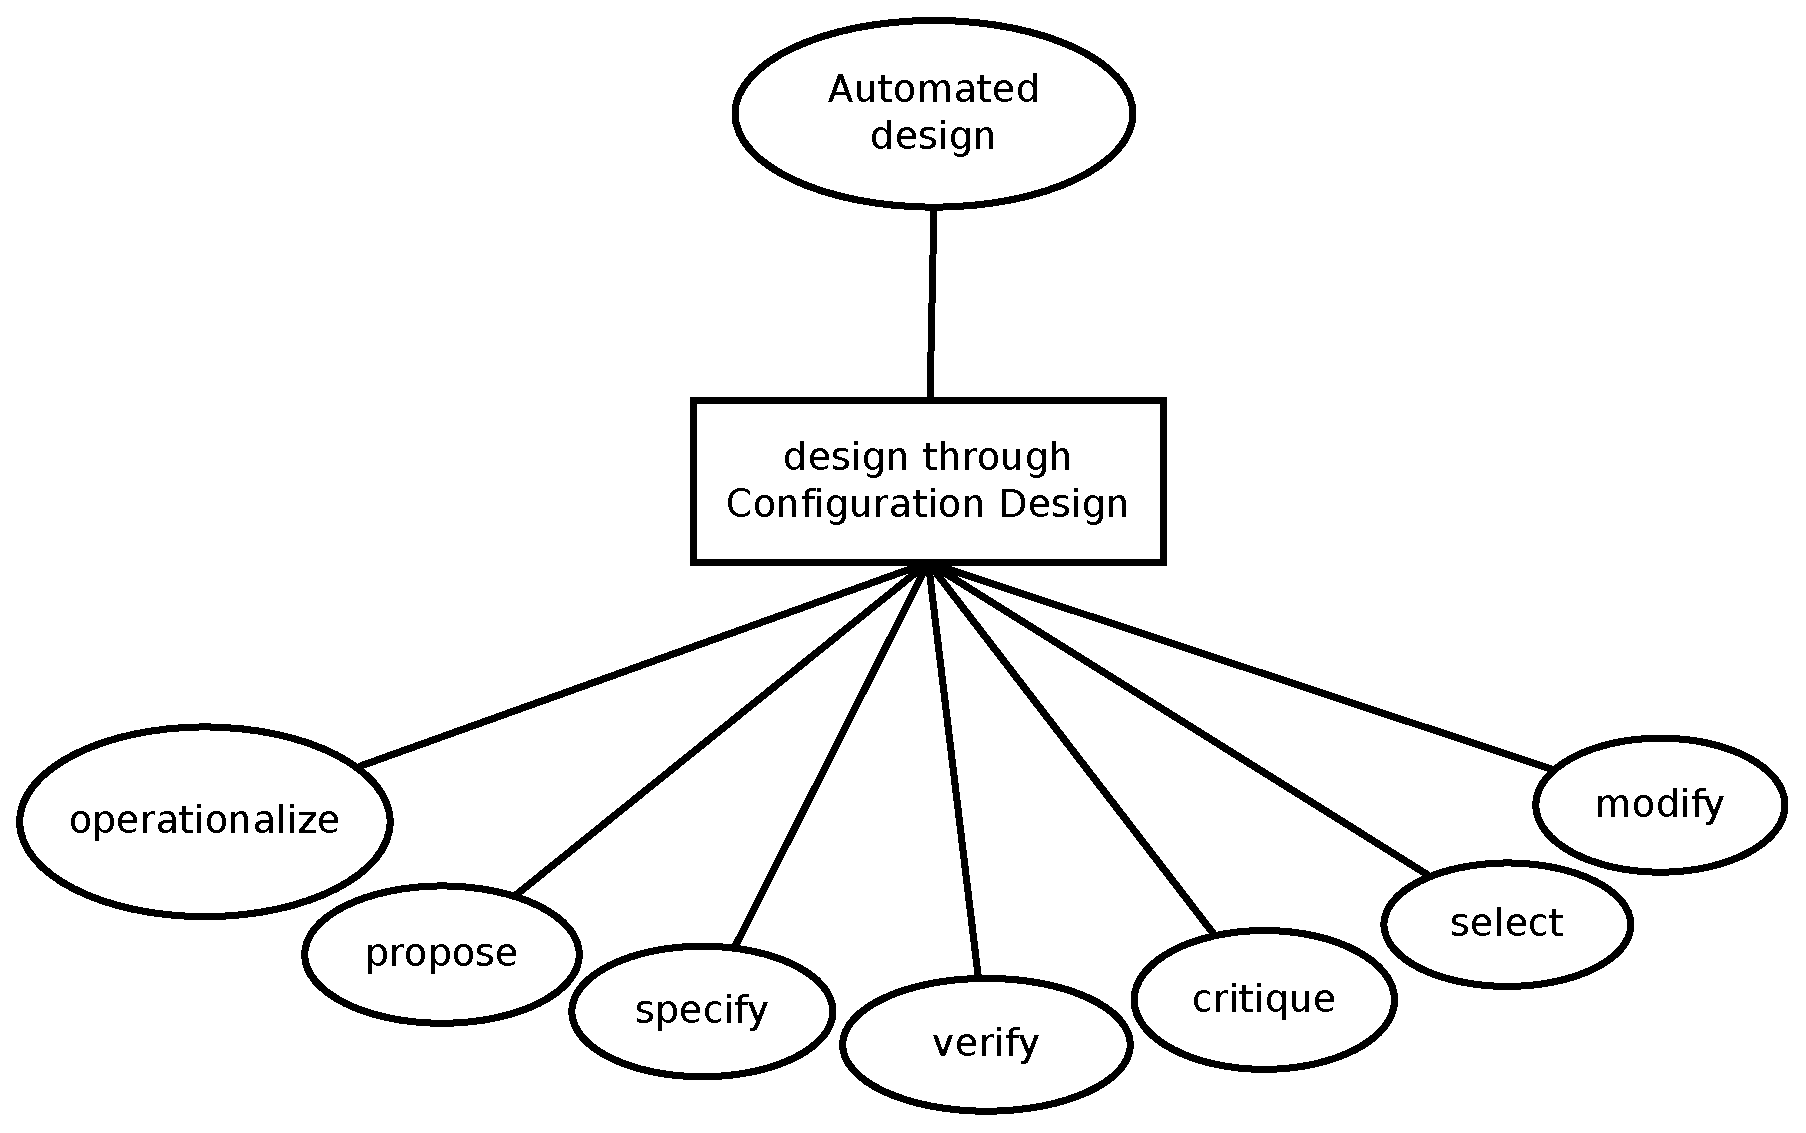
\includegraphics[height=7cm]{images/task_knowledge.eps}
\caption{Task knowledge}
\label{fig:taskknowledge}
\end{figure}

The ``propose and revise" method for configuration design presented in its original form in the textbook for the course has been slightly modified to obtain a method that reflects the needs of our software. The \textit{WHILE} loop to revise the the design has been postponed from a state of \textit{propose} to a state of \textit{verify}, and the internal \textit{REPEAT UNTIL} loop to select the actions has been integrated in the outer cycle. This way the method reflects exactly the intended steps to be realized in the software. 

\begin{lstlisting}[label=Task,caption=Task and task method description,breaklines=true]
TASK automated-design;
  ROLES:
    INPUT: request: "request for the design";
    OUTPUT: itinerary: "the resulting design";
END TASK configuration-design;

TASK-METHOD propose-and-revise;
  REALIZES: automated-design;
  DECOMPOSITION:
    INFERENCES: operationalize, propose, specify, verify, critique, select, modify;
  ROLES:
    INTERMEDIATE:
      preferences-and-requirements: "requirements and preferences to be preferably fulfilled";
      constraints: "requirements that have to be fulfilled";
      sketal-design: "set of slots to be filled";
      proposal: "a possible compilation of the sketal-design";
      customer-input: "set of new requirements or constraints";
      violation: "new constraints violated by the current design";
      truth-value: "boolean indicating the result of the verification";
      action-list: "ordered list of possible repair (fix) actions";
      action: "a single repair action";
      itinerary: "a new possible compilation of the sketal-design";
  CONTROL-STRUCTURE:
    operationalize(request -> preferences-and-requirements + constraints);
    specify(request -> sketal-design);
    propose(constraints + preferences-and-requirements + sketal-design -> proposal);
    itinerary := proposal ADD itinerary;
    WHILE verify(customer-input + itinerary -> truth-value + violation) IS truth-value == false DO
      critique(violation + itinerary -> action-list)
      select(action-list -> action)
      modify(itinerary + action -> itinerary)
      verify(itinerary + customer-input -> truth-value + violation);
    END WHILE
END TASK-METHOD propose-and-revise;
\end{lstlisting}

\clearpage
\section{Inference Knowledge}

As inference model we use a modified version of the Configuration design template, because given predefined components we need to find and assembly that satisfies the requirements. The inference model deriving from this task can be found in Figure~\ref{fig:inference}. \\
The standard inference model for the configuration design template (propose and revise) has been modified to better express the needs of our software, in a way that the system interacts directly with the client a second time right after the proposal phase: 
\begin{itemize}
\item Requirements have been transformed in Request
\item Soft and hard requirements have been transformed in ``preferences and requirements'' and ``constraints'' respectively
\item Extension has been changed into ``proposal''
\item Verify requires the direct input of the customer, since it's a verification of subjective correctness more than a verification of constraint violation. 
\item Design has been changed int ``itinerary'' for coherency purposes.
\end{itemize}
It has to be noted that the subsystem building the proposal, in the implementation of the system, does not permit a constraint violation, so the verification of the constrait has been removed because redundant.

\begin{figure}[h]
\centering
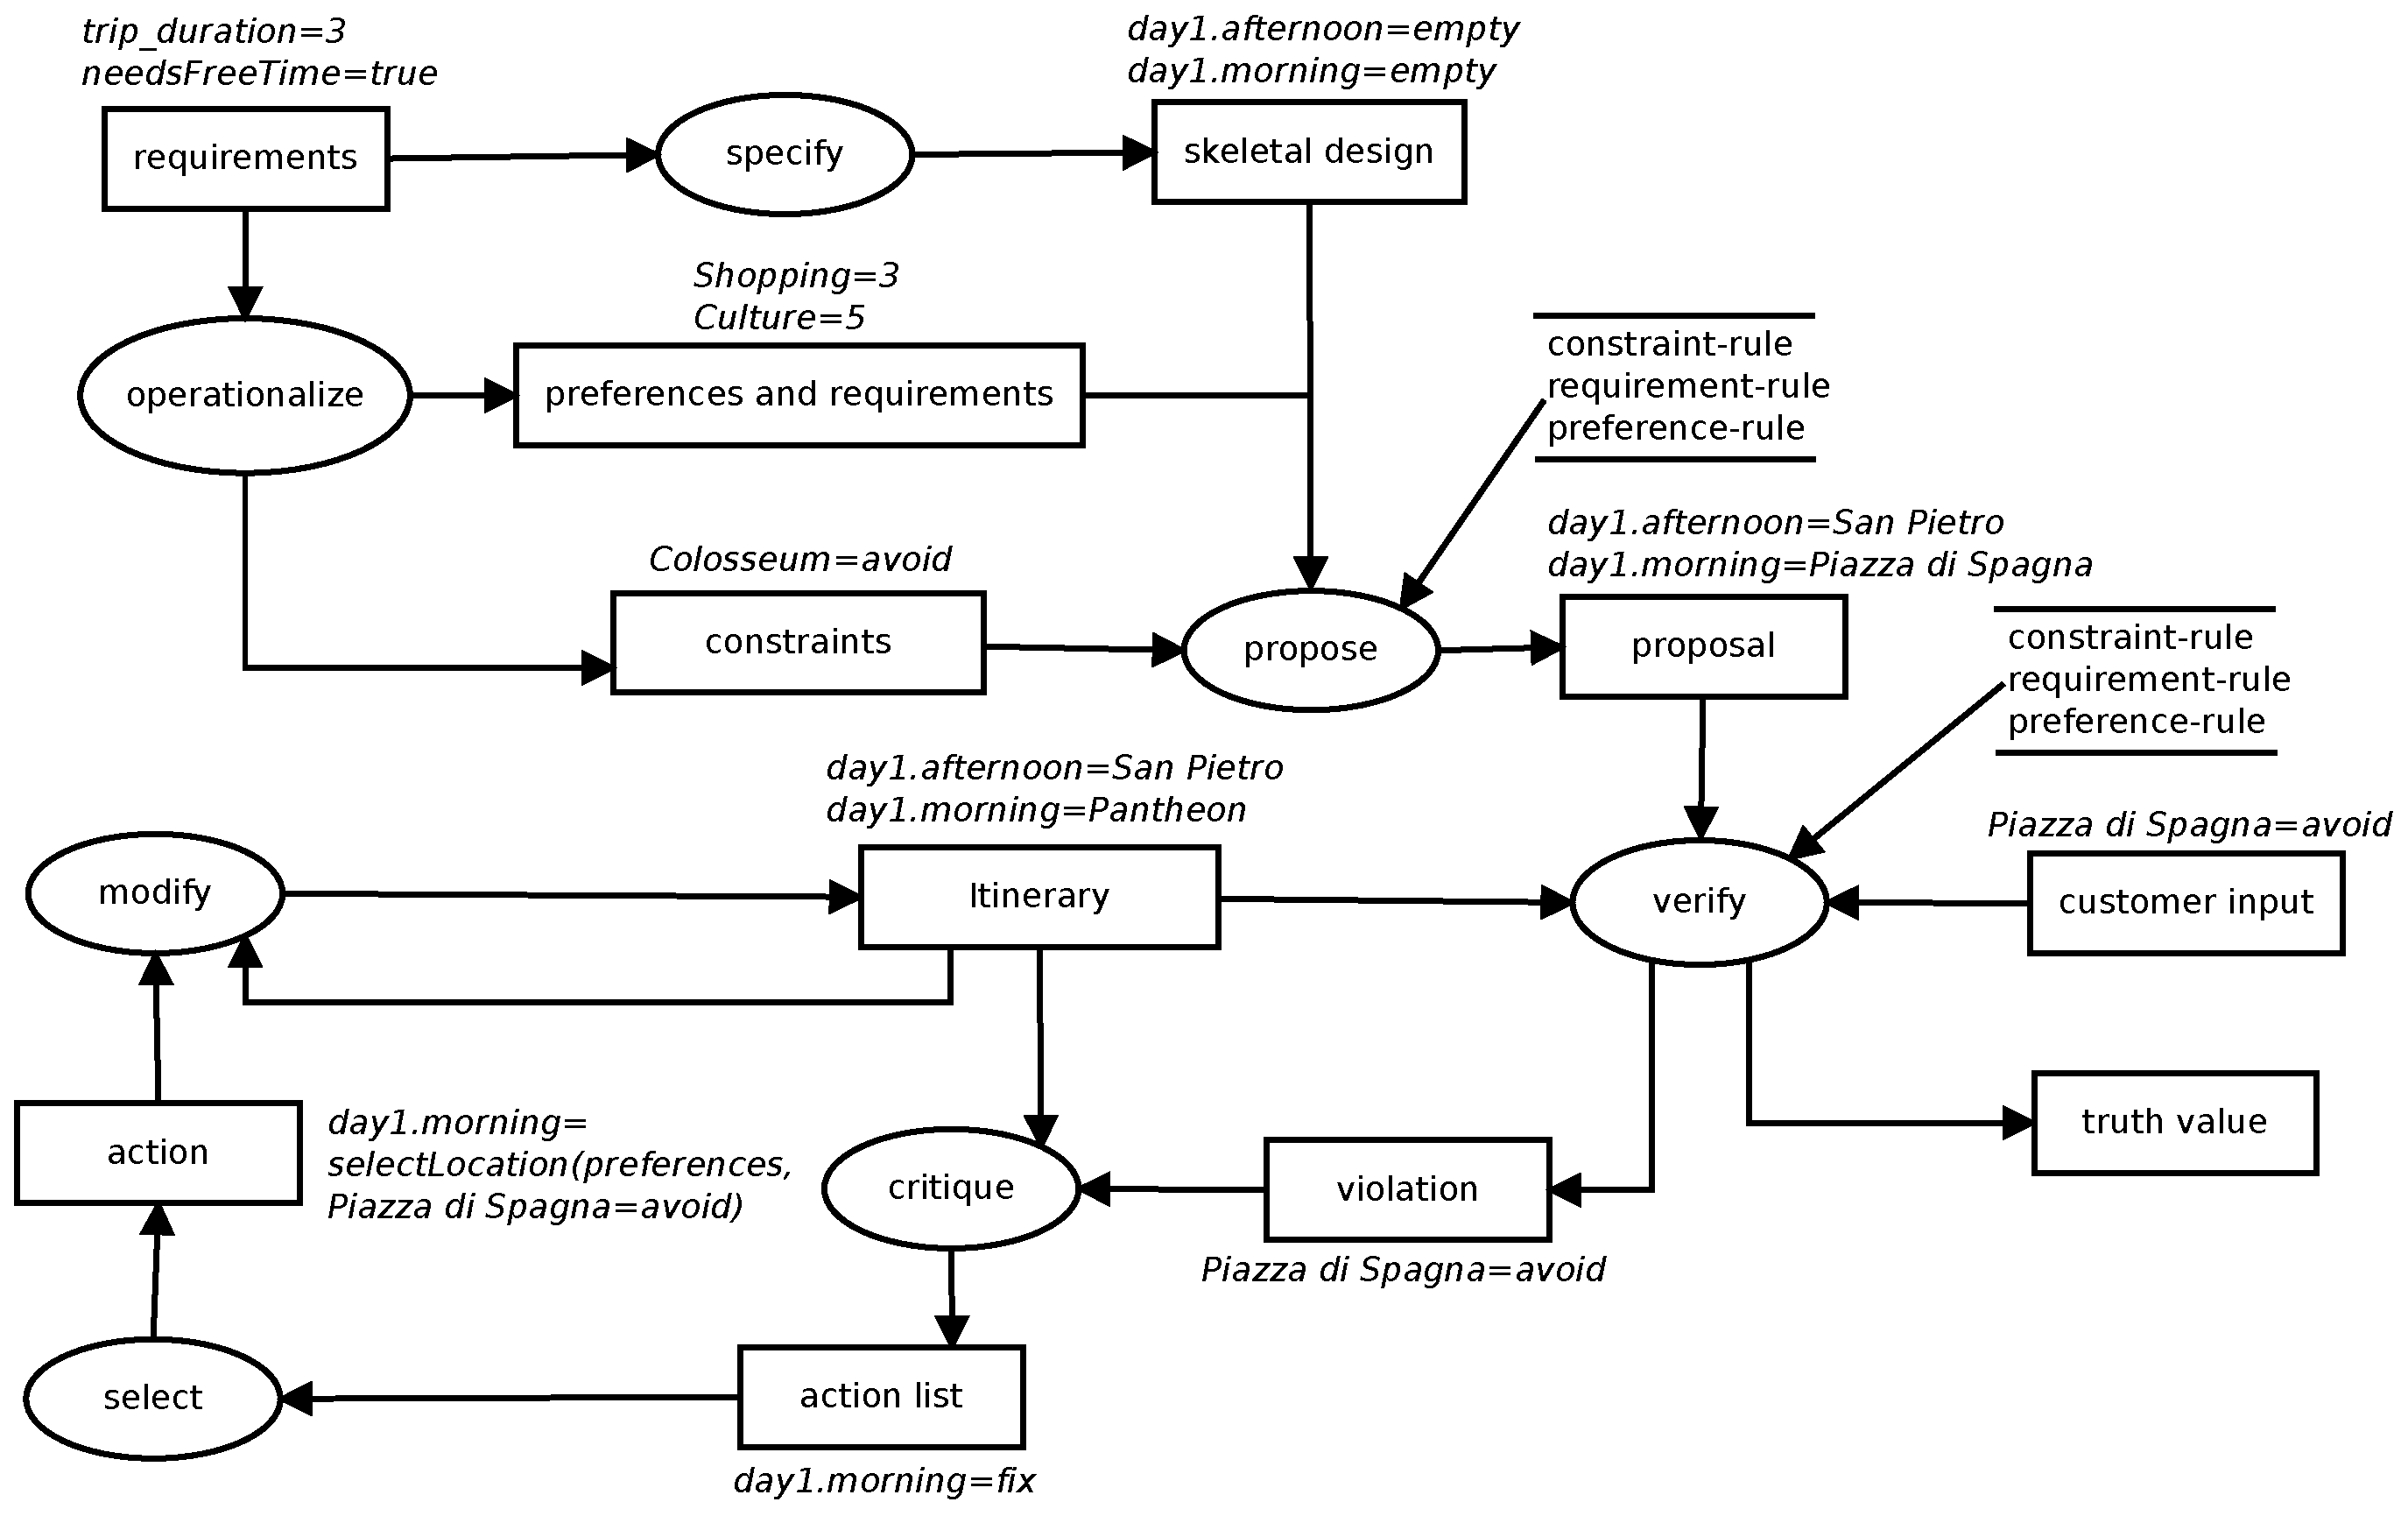
\includegraphics[width=\textwidth]{images/inference.eps}
\caption{Inference structure}
\label{fig:inference}
\end{figure}

\noindent
\begin{tabularx}{\textwidth}{| X | X | X | X |}
  \hline
Inference		& Input	& Output 	& Description \\ \hline \hline
specify		& request	& sketal design		& the function look-up the default sketal design: the basic structure of a trip day (heavy activity during the morning, relaxing afternoon, evening and meal).
\\ \hline 
   optionalize	& needs of the customers		& preferences, requirements, constraints	& the needs and desires are translated into preferences ("I would like to have time for shopping and visit many cultural places. I am not interested so much in food places"), requirements ("I want a quiet trip") and contraints ("In Rome I want to visit the \emph{Colosseum} and avoid \emph{Piazza di Spagna}"). 
\\ \hline
propose	& preferences and requirements, sketal design slots		& filled sketal design	& fill the slots of the sketal design with locations that fits the preferences and requirements.
\\
\hline
\end{tabularx}
\newpage
\noindent
\begin{tabularx}{\textwidth}{| X | X | X | X |}
\hline
verify		& contraints, extension design	& the list of violated contraints	& it checks with the help of the internal contraints and those supplied by the user whether the current configuration is internally consistent. If the verification fails, it produces the violated contraints as an additional output
\\ \hline
select 	& fix actions list		& fix action		& It simply selects an action from the fix actions list generated by the critique function.
\\ \hline
modify	& itinerary design, fix actions list		& fixed itinerary design		& it applies the fix actions to the design.
\\ \hline
critique	& itinerary, violations, customer's inputs	& fix actions list		& it creates a series of actions which will fix the violations of the contraints, following also the customer's inputs. For example the contraint "I absolutely want to visit the \emph{Colosseum}" will produce the action "Insert the \emph{Colosseum} into the itinerary".
\\ \hline
\end{tabularx}

\clearpage
\section{Domain knowledge}

%TODO: spiegare un po' le sorgenti di questo schema? Tipo risultati dell'intervista ecc? ma forse dobbiamo dirlo ben prima

\subsection{Domain schema}
The domain schema can be found in Figure~\ref{fig:ClassDiagram}

\begin{figure}[h]
\centering
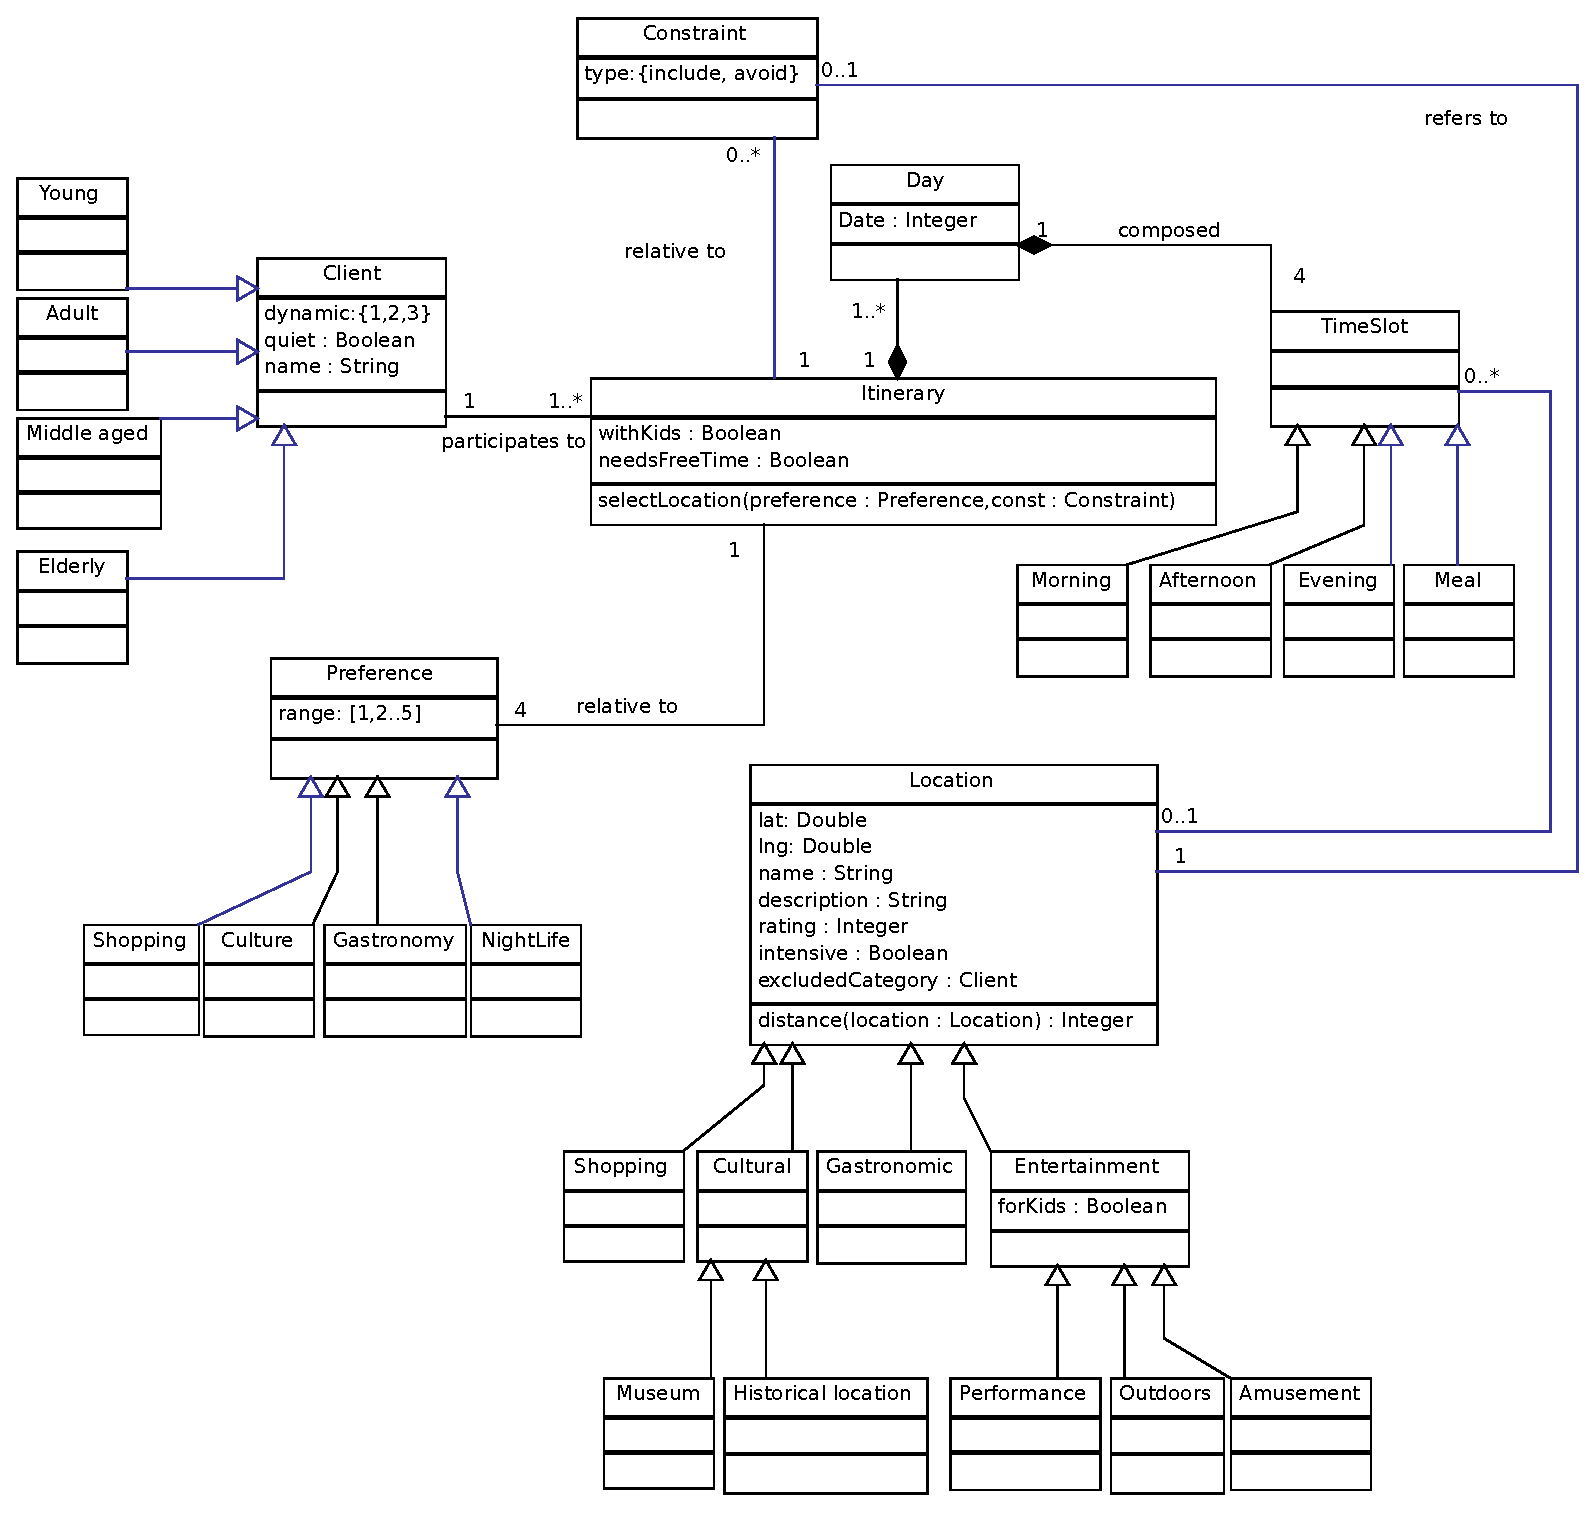
\includegraphics[width=\textwidth]{images/domain.eps}
\caption{Domain schema}
\label{fig:ClassDiagram}
\end{figure}

This schema seems complicated, for this reason every model is explained in the following list:
\begin{description}
  \item[Client] \hfill \\
  The client who goes to the travel agency. He could be a quite person who normally wants to visit a lot of things or very few (\emph{dynamic}). The clients are categorized by their age because some locations are not suitable for a people category (ex: elderly people in a climbing location).

  \item[Preference] \hfill \\
  Each client needs to specify a list of preferences, valued from 1 to 5, where 1 is ``I'm not so interested" and 5 is "I love to do it!". These preferences are related to the itinerary we want to create, consequently if the same clients wants to create another itinerary, it will specify again all the preferences he wants in this second trip.
  \item[Contraint] \hfill \\
  Each client needs to specify a list of contraints that have to be fulfilled. As for the \emph{Preference}, they are related to the single itinerary.
  \item[Itinerary] \hfill \\
  This represents the itinerary we want to create. It is composed by a fixed number of \emph{Day} and it is related to a \emph{Client} who has specified his own list of \emph{Contraint} and \emph{Preference}. If there will be kids in the itinerary, the system needs to select some \emph{Location} that could entertain them. This is a requirement as the \emph{needsFreeTime} attribute, which specifies that the clients needs to have some not scheduled time in the arrival city.\\
The method \emph{selectLocation} takes a list of \emph{Preference} and produces a list of \emph{Location} that could fit this preferences. 
  \item[Day] \hfill \\
  This describes a day of the itinerary.
  \item[Timeslot] \hfill \\
  A timeslot is a fixed part of a day. The division of the day came from the expert interview.
\item[Location] \hfill \\
  This model represents the point of interests that a customer could visit. The attribute \emph{rating} describes the quality of this place, \emph{intensive} describes if the place is not for quite people and \emph{excludedCategory} specifies if a client category is not suitable for the location (ex: elderly people in a climbing location). The method \emph{distance} takes two locations and returns the distance between them. It is useful in order to create the combination of locations to visit during a trip.
\end{description}

\subsection{Domain mapping}
\begin{figure}[H]
\centering
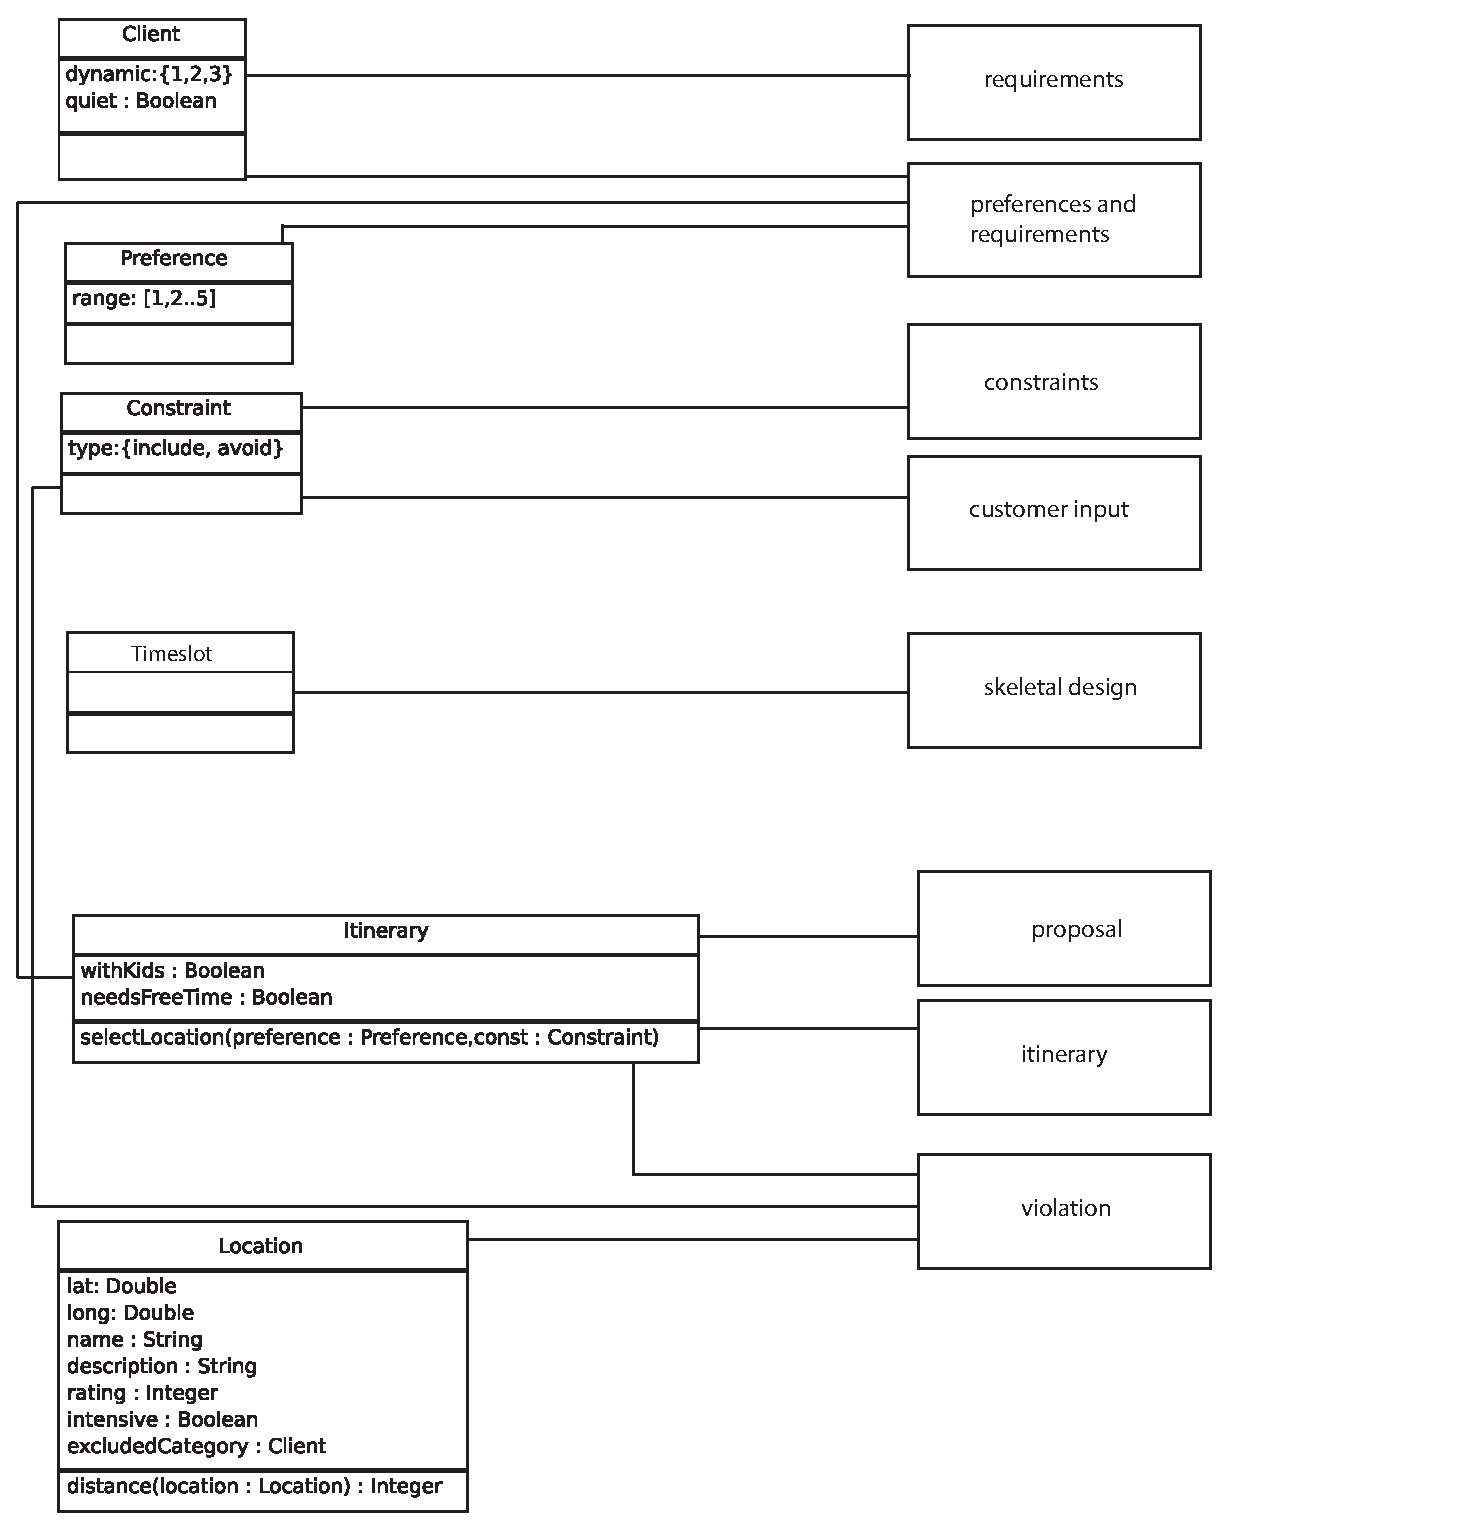
\includegraphics[width=\textwidth]{images/dom_VS_inference.eps}
\caption{Mapping between the domain model and the inference model}
\label{fig:MappingDomainInference}
\end{figure}
\noindent
\begin{tabularx}{\textwidth}{| X | X | X | X |}
\hline 
\textbf{Knowledge Role} & \textbf{Type} & \textbf{Domain Mapping}
\\ \hline \hline
request    &   dynamic  & Client
\\ \hline
skeletal design  & static    & Timeslot
\\ \hline
preferences and requirements  & dynamic    & Client, Itinerary, Preference
\\ \hline
constraints  & dynamic    & Constraint
\\ \hline
customer input  & dynamic    & Constraint
\\ \hline
proposal  & dynamic    & Itinerary
\\ \hline
itinerary  & dynamic    & Itinerary
\\ \hline
violation  & dynamic    & Constraint, Location %TODO: CONTROLLARE SCHEMA
\\ \hline
constraint-rule  & static    & Constraint
\\ \hline
preference-rule  & static    & Preference
\\ \hline
requirement-rule  & static    & Client, Itinerary
\\ \hline
\end{tabularx}

\subsection{Rule types}

\begin{lstlisting}[label=Rules,caption=Rules,breaklines=true]
RULE TYPE constraint-rule;
    DESCRIPTION: "rule stating the relation between client and the choice for a location in the itinerary, by means of defining strict boundaries that must be respected.";
ANTECEDENT: Client;
CONSEQUENT: Itinerary;
CONNECTION-SYMBOL: restricts;
END RULE-TYPE constraint-rule;

RULE TYPE requirement-rule;
    DESCRIPTION: "rule stating the relation between the client and the choice for a location in the itinerary, by means of defining boundaries that should be respected.";
ANTECEDENT: Client;
CONSEQUENT: Itinerary;
CONNECTION-SYMBOL: requires;
END RULE-TYPE requirement-rule;

RULE TYPE preference-rule;
    DESCRIPTION: "rule stating the relation between the client and the choice for a location in the itinerary, by means of defining preferences that could be satisfied with probability X (calculated on the input values) .";
ANTECEDENT: Client;
CONSEQUENT: Itinerary;
CONNECTION-SYMBOL: prefers-with-probability;
END RULE-TYPE preference-rule;
\end{lstlisting}


\noindent
Here are presented also some example in order to better understand all the rule types.

\begin{lstlisting}[label=Rules,caption=The client wants to include a destination into the itinerary.,breaklines=true,mathescape=true]
client.constraint.location.name$=$A AND client.constraint.type$=$include
RESTRICTS
$\exists$itinerary.day.timeslot, timeslot.location.name$=$A;
\end{lstlisting}



%TODO!!!!
\begin{lstlisting}[label=Rules,caption=The client is a quite person,breaklines=true,mathescape=true]
client.quiet=true, client.needsFreeTime=true, client.active=1
REQUIRES
itinerary.day.timeslot.location, location.intensive=false;
itinerary.day.timeslot, timeslot.location=NULL;
$\sum_{i=1}^{n-1}$i.distance(i+1) $<\delta$, $\forall$i $\in$ location;
\end{lstlisting}




\begin{lstlisting}[label=Rules,caption=The client expresses four preferences with four ranges (from 1 to 5). The method selectLocation will compose the itinerary selecting the locations that fits the preferences. For example it could select 3 shopping\, 1 gastronomy and 1 cultural locations.,breaklines=true,mathescape=true]
Var A, B, C, D: client.preference;
Var E: client.constraint;
A.type=shopping AND A.range=x
B.type=cultural AND B.range=y
C.type=gastronomy AND C.range=w
D.type=nightlife AND D.range=z
E.type = avoid AND E.location = Colusseum
PREFERS-WITH-PROBABILITY
$\forall$itinerary.day.timeslot, timeslot.location=selectLocation(A, B, C, D, E);
\end{lstlisting}

\subsection{Knowledge Base}

The Knowledge base can be seen in Figure~\ref{fig:knowledgebase}.

\begin{figure}[H]
\centering
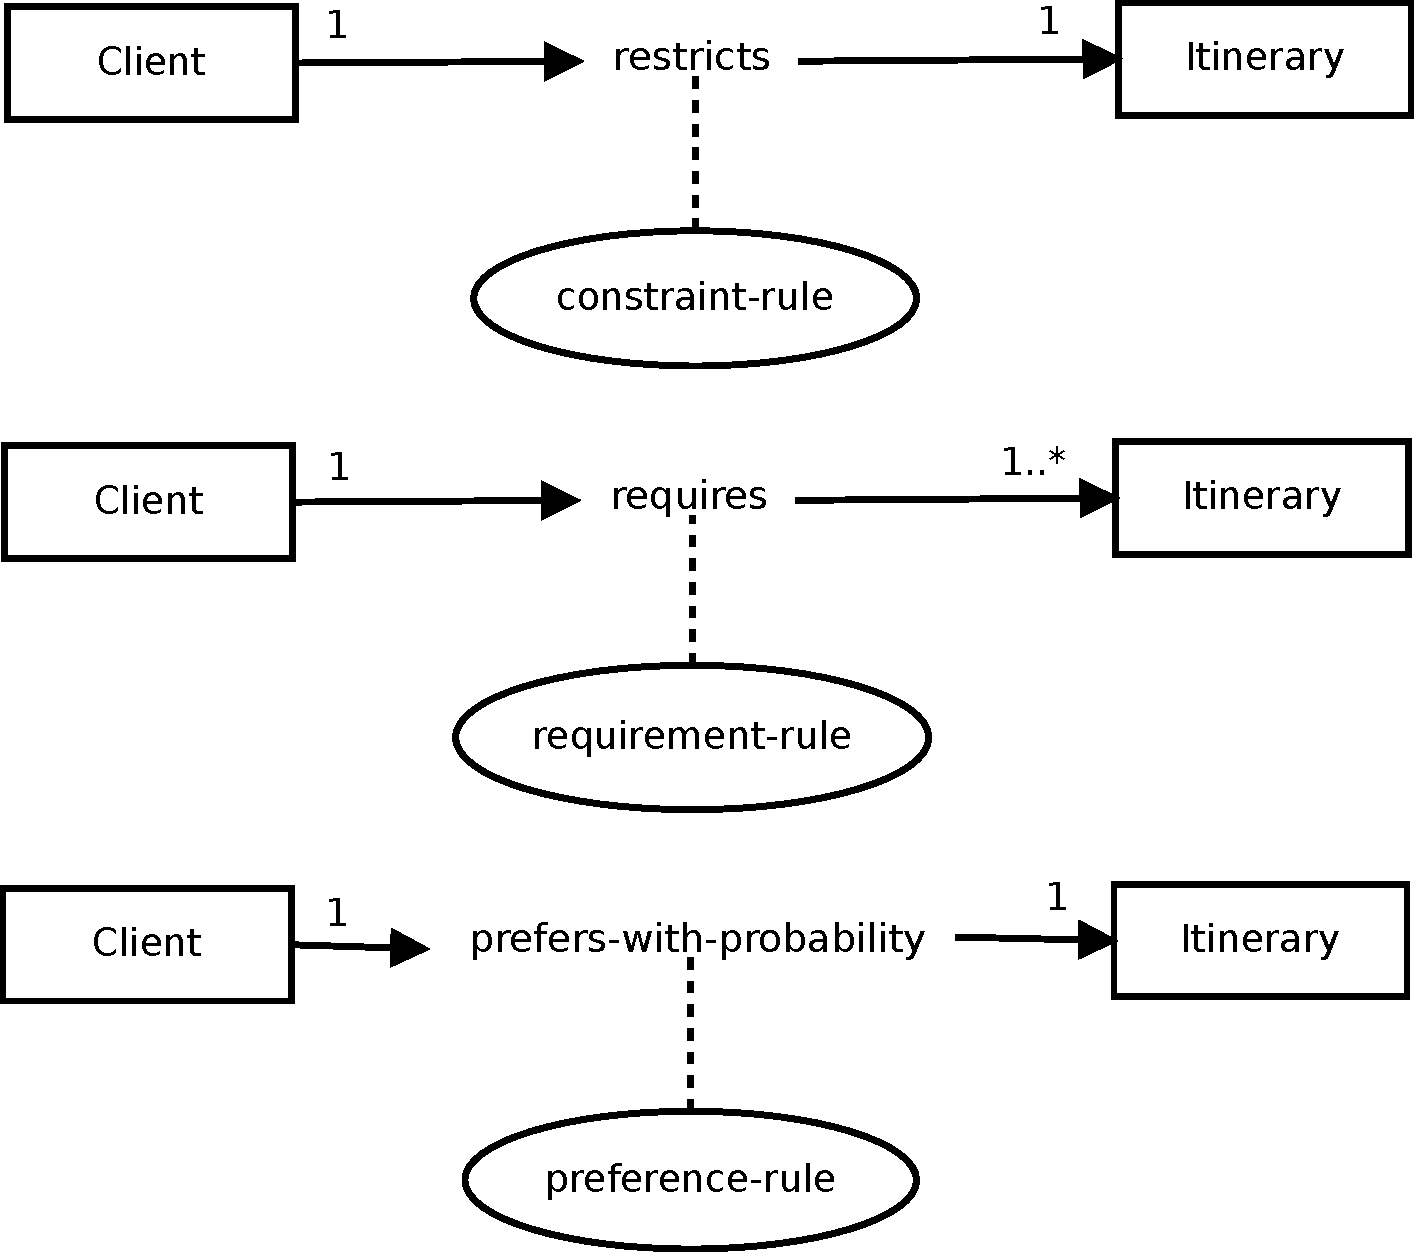
\includegraphics[height=7cm]{images/knowledge_base.pdf}
\caption{Knowledge base}
\label{fig:knowledgebase}
\end{figure}



\section{Scenarios}

\subsection{Scenario 1}

Rose, a 76 years old lady would like to visit Rome for three days with her nephew John who is ten years old. She would like to have her trip planned but with the possibility to explore the city on her own. 

\subsubsection{Interview}

\begin{description}
  \item[Are you used to walk long distances?] \hfill \\
  Not at all, I usually don't walk a lot.
  \item[In a scale from one to five, how do you enjoy shopping?] \hfill \\
  I really love to do shopping, so five!
  \item[In a scale from one to five, how do you enjoy cultural places?] \hfill \\
  I am going to Rome, so four!
  \item[In a scale from one to five, how do you enjoy nightlife?] \hfill \\
  Have you looked at me? 1!
  \item[In a scale from one to five, how much would you like to try new restaurants?] \hfill 
  I guess... I don't know, 3?
  \item[Is there anything that you'd absolutely like to see?] \hfill \\
  Yes, I've never seen the Colosseum.
  \item[Is there anything that you have already seen or don't want to see?] \hfill \\
  Not really, everything is fine.
\end{description}

The travel agent while is interviewing the customer, inserts the acquired data into the system through graphic interface.

\subsubsection{Operazionalize}
The system once it receives the request divides them into three categories: requirements, preferences and constraints.

\begin{lstlisting}[breaklines=true,mathescape=true]
REQUIREMENTS:
  client.quiet = true
  client.dynamic = 1
  itinerary.withKids = true
  itinerary.needsFreeTime = true
  VAR a,b,c: day;
  a.date = "14/05/2014"
  b.date = "15/05/2014"
  c.date = "16/05/2014"
PREFERENCES:
  VAR a,b,c,d : preference;
  a.type = shopping
  a.range = 5
  b.type = culture
  b.range = 4
  c.type = nightlife
  c.range = 1
  d.type = gastronomy
  d.range = 3
CONSTRAINTS:
  constraint.location.name = Colosseum
  constraint.type = include
\end{lstlisting}

\subsubsection{Specify}
The system reads the request and compiles the skeletal design, an empty itinerary containing only the structure of the days.

\begin{lstlisting}[breaklines=true,mathescape=true]
REQUIREMENTS:
  VAR a,b,c: day;
  a.date = "14/05/2014"
  b.date = "15/05/2014"
  c.date = "16/05/2014"
SKELETAL-DESIGN:
  NEW-ITINERARY(a.date, c.date)
\end{lstlisting}

\subsubsection{Propose}
The system processes the request using the knwoledge rules and returns a first version of the itinerary.

\begin{lstlisting}[breaklines=true,mathescape=true]
ITINERARY:
  VAR a,b,c: day;
  a.date = "14/05/2014"
  b.date = "15/05/2014"
  c.date = "16/05/2014"
  a.morning = Colosseum
  a.afternoon = Shopping mall "I gladiatori"
  a.meal = Parolaccia
  a.evening = Fontana di Trevi
  b.morning = Villa Borghese
  b.afternoon = Outlet shoes Roma
  b.meal = Pizzeria da Matteo
  b.evening = Piazza di Spagna
  c.morning = EMPTY
  c.afternoon = EMPTY 
  c.evening = Piazza del Popolo
  
\end{lstlisting}

\subsubsection{Verify}
The system passes the itinerary to the TA through the GUI. The TA asks the Client for a confirmation or the need for modification.

\begin{description}
  \item[This is a possible itinerary, do you have any modifications you want to do?] \hfill \\
  Yes please, I don't need shoes.
\end{description}

\subsubsection{Critique}
Based on the Client feedback, the system builds an action list of modifications

\begin{lstlisting}[breaklines=true,mathescape=true]
ACTION-LIST:
  contraint.location = Outlet shoes Roma
  constraint.type = avoid
  
\end{lstlisting}

\subsubsection{Select}
The system chooses one action at the time for the itinerary to be modified

\begin{lstlisting}[breaklines=true,mathescape=true]
ACTION:
  contraint.location = Outlet shoes Roma
  constraint.type = avoid
  
\end{lstlisting}

\subsubsection{Modify}
The system modifies the itinerary accordingly to the selected action.

\begin{lstlisting}[breaklines=true,mathescape=true]
ITINERARY:
  VAR a,b,c: day;
  a.date = "14/05/2014"
  b.date = "15/05/2014"
  c.date = "16/05/2014"
  a.morning = Colosseum
  a.afternoon = Shopping mall "I gladiatori"
  a.meal = Parolaccia
  a.evening = Fontana di Trevi
  b.morning = Villa Borghese
  b.afternoon = Le Piramidi
  b.meal = Pizzeria da Nando
  b.evening = Piazza di Spagna
  c.morning = EMPTY
  c.afternoon = EMPTY 
  c.meal = EMPTY
  c.evening = Piazza del Popolo
  
\end{lstlisting}

\subsubsection{Verify}
The system passes the itinerary to the TA through the GUI. The TA asks the Client for a confirmation or the need for modification.

\begin{description}
  \item[This is a possible itinerary, do you have any modifications you want to do?] \hfill \\
  No, the itinerary is fine.
\end{description}

\subsection{Scenario 2}
Richard a 30 years old guy, would like to visit Rome for two days alone.

\subsubsection{Interview} 

\begin{description}
  \item[Would you consider yourself a quite person or ready to have some fun?] \hfill \\
  Definitely have fun.
  \item[Are you used to walk long distances?] \hfill \\
  Yeah.
  \item[In a scale from one to five, how do you enjoy shopping?] \hfill \\
  Not that much I only need to buy some souvenirs, 1.
  \item[In a scale from one to five, how do you enjoy cultural places?] \hfill \\
  I am going to Rome, so four!
  \item[In a scale from one to five, how do you enjoy nightlife?] \hfill \\
  I don't know... 5?
  \item[In a scale from one to five, how much would you like to try new restaurants?] \hfill 
  I definitely like to eat, 5.
  \item[Is there anything that you'd absolutely like to see?] \hfill \\
  Yes, I've never seen the EUR.
  \item[Is there anything that you have already seen or don't want to see?] \hfill \\
  I'm not interested in San Pietro.
\end{description}

The travel agent while is interviewing the customer, inserts the acquired data into the system through graphic interface.

\subsubsection{Operazionalize}
The system once it receives the request divides them into three categories: requirements, preferences and constraints.

\begin{lstlisting}[label=Rules,caption=Domain instance of the data inserted into the system,breaklines=true,mathescape=true]
REQUIREMENTS:
  client.quiet = false
  client.dynamic = 3
  itinerary.withKids = false
  itinerary.needsFreeTime = false
  VAR a,b,c,d: day;
  a.date = "14/05/2014"
  b.date = "15/05/2014"
PREFERENCES:
  VAR a,b,c,d : preference;
  a.type = shopping
  a.range = 1
  b.type = culture
  b.range = 4
  c.type = nightlife
  c.range = 5
  d.type = gastronomy
  d.range = 5
CONSTRAINTS:
  VAR a,b : constraint;
  a.location.name = EUR
  a.type = include
  a.location.name = San Pietro
  a.type = avoid
\end{lstlisting}

\subsubsection{Specify}
The system reads the request and compiles the skeletal design, an empty itinerary containing only the structure of the days.

\begin{lstlisting}[breaklines=true,mathescape=true]
REQUIREMENTS:
  VAR a,b,c: day;
  a.date = "14/05/2014"
  b.date = "15/05/2014"
SKELETAL-DESIGN:
  NEW-ITINERARY(a.date, b.date)
\end{lstlisting}

\subsubsection{Propose}
The system processes the request using the knwoledge rules and returns a first version of the itinerary.

\begin{lstlisting}[breaklines=true,mathescape=true]
ITINERARY:
  VAR a,b,c: day;
  a.date = "14/05/2014"
  b.date = "15/05/2014"
  a.morning = Colosseum
  a.afternoon = Pantheon
  a.meal = Parolaccia
  a.evening = Discoteca el muendo
  b.morning = Villa Borghese
  b.afternoon = EUR
  b.meal = Pizzeria da Matteo
  b.evening = Discoteca Roma
  
\end{lstlisting}

\subsubsection{Verify}
The system passes the itinerary to the TA through the GUI. The TA asks the Client for a confirmation or the need for modification.

\begin{description}
  \item[This is a possible itinerary, do you have any modifications you want to do?] \hfill \\
  No, the itinerary is fine.
\end{description}




\clearpage
\section{Communication Knowledge}
The communication model specifies the information exchange between tasks carried out by different agents. It has been designed as an Activity Diagram where the name of the interaction corresponds to the type of communication happensing between the agents in the connected lanes.\\
It has to be noted that the only task knowledge intensive is ``Automatically build the itinerary'' carried out by the automated system \textit{easyAround}.\\
The mapping between the activities in the communication model and the inference model is schematized as follows:
\begin{itemize}
\item ``operationalize'' corresponds to ``differentiate constraints, requirements and preferences''
\item ``specify'' and ``propose'' are mapped to ``automatically build the itinerary''
\item ``verify'' corresponds to ``obtain feedback''
\item ``critique'' corresponds to ``edit itinerary''
\end{itemize}
Our Communication Process can be see in Figure~\ref{fig:CommunicationDiagram}.

\begin{figure}[h]
\centering
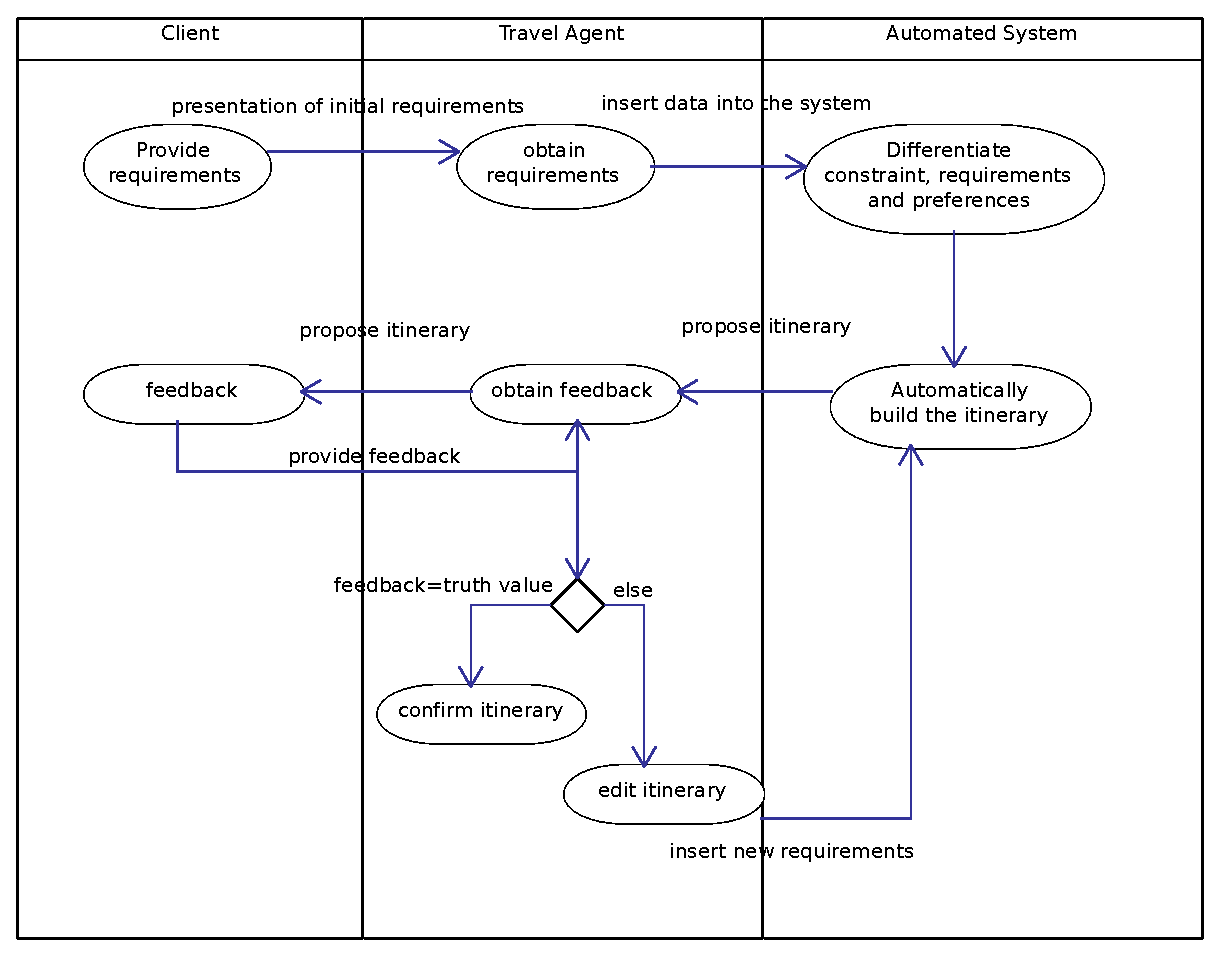
\includegraphics[width=\textwidth]{images/communication.eps}
\caption{Communication process}
\label{fig:CommunicationDiagram}
\end{figure}

\worksheet{CM-1}{Transaction Descritpion worksheets}

\worksheet{CM-2}{Information exchange specification}

\clearpage
\section{Design Knowledge}

\worksheet{DM-1}{System Architecture}

\worksheet{DM-2}{Target implementation platform}

\newpage
\section{Implementation}
\subsection{Role of the CommonKADS model set in the implementation}
\subsection{Reflection on problems and results}
\subsection{Spiral Approach}

\newpage

\appendix
\section{Design Knowledge}

In preparation for the interview with the expert we listed a series of concepts to be clarified in order to better structure the application domain. 

\begin{enumerate}
  \item Target of the application: which kind of customer the application is more suitable for;
  \item Subcategories of the target: is it possible to recognize different subcategories in the target that correspond to different needs for the creation of an itinerary;
  \item Locations of interest: understand which categories of locations can be created and in which way they can be matched with the customer's preferences;
  \item Composition of the itinerary: understand the basic structure of an itinerary, and whether it can be composed automatically.
\end{enumerate}

The interviewing techniques applied were mainly two: problem solving (the interviewer poses himself as a customer and watches the expert "in action") and 20-Questions (the interviewer thinks about a destination for an hypothetical itinerary and the expert needs to guess which one it is). Relatively to the categorization of the locations, it has also been used the "Card sorting".
The results of the interview were satisfying:

\begin{enumerate}
  \item The target of the application are the "lonely travelers", people who prefer traveling on their own, at most with their family.
  \item It has been concluded that the target can be divided in four age-based category, such as "Young" (18-30), "Adults" (30-40), "Middle aged" (40-60), "Elderly" (60+). Relating to these categories the aspects that change the most are: need for entertainment, need for quiet, free time available, amount of time spent walking.
  \item The locations can be divided in four main categories such as "shopping", "gastronomy", "cultural" and "entertainment"; of these, "cultural" can be divided in "historical locations" (such as monuments) and "museums", and "entertainment" can be divided in "amusement" (such as clubs, pubs and discos), "performance" (such as cinemas, theatres, \ldots)  and "outdoor" (such as amusement parks or gardens).
  \item It has been concluded that the itinerary can be seen as an aggregation of days, which in turn have a basic fixed structure. 
\begin{description}
  \item[Morning] non intensive activity (monuments, gardens\ldots);
  \item[Afternoon] intensive activity (museums, shopping\ldots);
  \item[Evening] the intensity of the activity depends on personal preferences.
\end{description}
\end{enumerate}

From the interview emerged an aspect not considered before, that is to say the presence of kids. The expert pointed out that in case a child is present, the itinerary is to be built as usual but having care of including children activities every once in a while.
A constraint to be considered is the fact that the customer can request a location to be included or excluded from the itinerary.




\end{document}
